%-------------------------------------------------------
% Gamification Techniques
%-------------------------------------------------------
\section{What Gamification is}

Gamification consists of using game developing techniques in
non-game environments, such as social networks [16], e-health, e-commerce, and educational systems. The techniques and resources used in digital games have elements
capable of (i) motivate users,(i) hold their interest, and (iii) challenge them
to solve problems. In gamification approaches, these elements are
not the center of the system, instead these elements have the purpose of attract users and motivate them to keeping using it [28]. Foursquare application (Figure 1-b) is an
example of a gamified system. Foursquare is a location-based
social network, which reached one billion “check-ins” in 2011 [ref].
Foursquare allows users to check-in at venues using a device specific
front-end to the application (e.g., mobile website), each
check-in might award the user with user-points or “badges”. 
\textit{Explicar pointification, 
Argumentar que evoluiu agora trend personalização.}

% Gamification
\begin{figure}[h!]
\caption{Gamification.}
\centering

\includegraphics[width=0.3\textwidth]{Work_In_Progress}
\label{fig:work_in_progress}
\end{figure}

\subsection{What Gamification is not}

Here, we will define some concepts related to the term "game". The following discussion is not comprehensive, and it is only intended to clarify and narrow down our definition of gamification. A more comprehensive and deep discussion can be found in \citeauthor{Deterding2011}.

\begin{itemize}
\item Gamification is not Playful design or gameful design:
\end{itemize}

Playful design is using game-based aesthetics or limited usability
based on game elements in non-game contexts with the purpose of
drawing the user's attention [1]. These elements are used to amuse
users and cause an emotional response. One successful example is
Twitter’s page knows as “Fail Whale” (Figure 1-a). Whenever
there is an overload on the servers, instead of a boring page with
some standard error message, users are presented with a drawing of
a dozen birds, twitters, trying to lift a whale.

% Playful design or gameful design
\begin{figure}[h!]
\caption{Playful design or gameful design.}
\centering

\includegraphics[width=0.3\textwidth]{Work_In_Progress}
\label{fig:work_in_progress}
\end{figure}

\begin{itemize}
\item Gamification is not Serious games:
\end{itemize}

Serious games are games designed for non-recreational
environments and for educational purposes [16]. The term
“serious” is employed because these games can focus on areas as
diverse as economics, education, health, industry, military,
engineering, and politics. In environments created by applying
serious game concepts, it is possible to simulate real-world
situations without incurring in eventual costs and risks. The main
goal of this sort of training-environment is to convey information
to the user [31]. The Virtual Incident Management Training System
(Figure 1-c) is a multiplayer training environment designed for
training professionals that need to act swiftly in case of accident on
highways, such as paramedics and policemen [37].

% Serious game
\begin{figure}[h!]
\caption{Serious games.}
\centering

\includegraphics[width=0.3\textwidth]{Work_In_Progress}
\label{fig:work_in_progress}
\end{figure}

\begin{itemize}
\item Gamification is not Video games or digital games:
\end{itemize}

Video Games or Digital Games are systems in which users are
engaged in resolving abstract conflicts and challenges, under
predetermined rules [36]. In this scenario the game continuously
offers interactivity and feedback to the user, which often result in
an emotional reaction. Figure 1-d shows a screenshot of the game
New Super Mario Bros.Wii\copyright whose main character, Mario, is
considered one of the most iconic video game characters.

% Video games or Digital games
\begin{figure}[h!]
\caption{Video games or Digital games.}
\centering

\includegraphics[width=0.3\textwidth]{Work_In_Progress}
\label{fig:work_in_progress}
\end{figure}

It is worth to point out that the current thesis focus on covering
research that explicitly match our definition of Gamification.
Therefore, we are not considering research based on serious games,
video games, playful design and other uses of game concepts in
educational contexts.

%-------------------------------------------------------
% Game Design Elements
%-------------------------------------------------------
\section{Game Design Elements}
\sigla{GDE}{Game design elements} is a term used to cover a broad list of game mechanics, dynamics, and aesthetics used in the design and development of games \cite{The_Gamification_of_Learning_and_Instruction,Gamification_of_Collaborative_Learning}. In the gamification process, these elements work as motivational \textit{affordances} to deliver gameful experiences to the users, and as a consequence, trying to influence their behavior \cite{Does_Gamification_Work}. 
A coarse-grained definition of the main categories of GDE is as it follows: 

\begin{itemize}
\item \textbf{Mechanics} They define the rules, actions and behaviors allowed in the game, and they are characterized by game components at the level of data representation and algorithms:
\subitem Examples: Rules, goals (objectives), levels, number of players. 
\item \textbf{Dynamics} characterize the run-time behavior of the mechanics reacting on player inputs;
\subitem Examples: Feedback, conflict, competition, cooperation, time pressure.
\item \textbf{Aesthetics} characterize the interaction with the game system (i.e., input-output and vice versa).
\subitem Examples: Sensation, fantasy, narrative, challenge, fellowship, discovery, expression.
\end{itemize}

According to \citeauthor{hunicke2004}, starting from the designer’s perspective,
the mechanics rise the dynamic system behavior, which in turn produces aesthetic experiences that will be consumed by the player.
However, from the player’s perspective, aesthetics set the \textit{tone} of the experience as a direct result of player's reaction to the dynamics, in turn, dynamics are paced by the available mechanics. For this reason it is important to have both perspectives in the radar, and neglecting none of them.

% Video games or Digital games
\begin{figure}[h!]
\caption{Designers and players have different, but linked, perspectives of the game. Adapted from \cite{hunicke2004}}
\centering
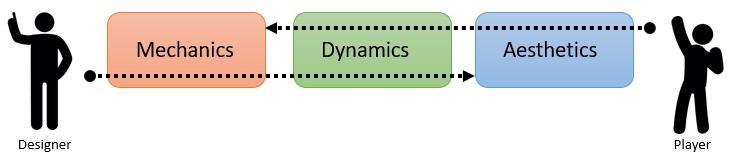
\includegraphics[width=0.8\textwidth]{mda_views}
\label{fig:mda_views}
\end{figure}

\textbf{Challenge} is an example of aesthetic element. 
It is a powerful element since it poises an obstacle between the player and the reward/victory. 
For instance, challenge can be created by the dynamic \textbf{time pressure}, where the player has limited time to accomplish a task. 
In turn, time pressure to exist depends of mechanics such as \textbf{rules specification} (e.g., how much time does the player have?) and the \textbf{rules implementation} (e.g., algorithms and data). 
As an example of the usage of such approach in a game, we can cite the Super Mario game franchise. In many games of the franchise, the character Mario needs to reach the end of the stage before running out of time otherwise the player will fail the challenge (Figure \ref{fig:mda}). Figure \ref{fig:duolingo} shows an example of the same usage, challenge based on time pressure, however in a non-game application. The application in question is Duolingo, a well known free language-learning platform. Duolingo is a successful example of how gamification can be skillfully applied to a system \cite{Huynh2016}. In the example, the learner needs to complete a task in an specific amount of time to be rewarded. 

% https://www.quora.com/How-effective-is-Duolingo-in-learning-a-language

% Figura Mario
\begin{figure}[h!]
\caption{Usage example of "challenge based on time pressure" in a game.}
\centering
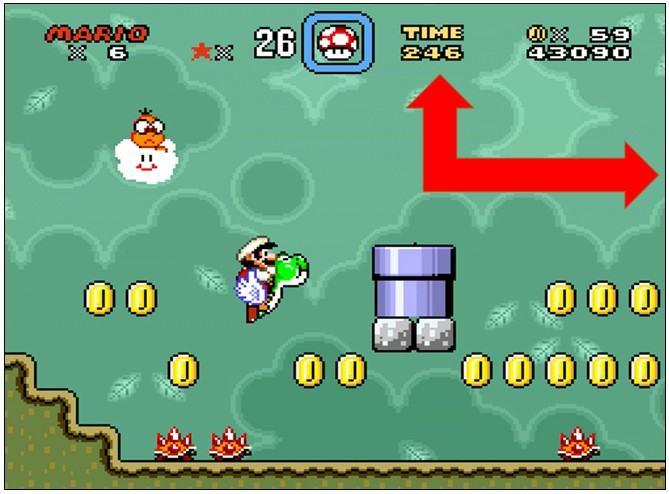
\includegraphics[width=0.4\textwidth]{mda}
\label{fig:mda}
\end{figure}

% Figura Duolingo
\begin{figure}[h!]
\caption{Usage example of "challenge based on time pressure" in a gamified application.}
\centering
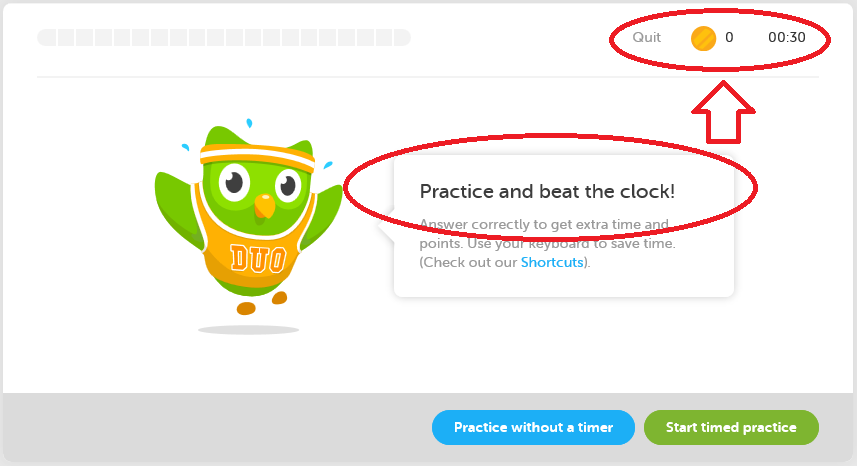
\includegraphics[width=0.6\textwidth]{duolingo2}
\label{fig:duolingo}
\end{figure}

GDE have been exhaustedly discussed in the gamification literature \cite{kapp2012gamification,robinson2013preliminary,werbach2012win,zichermann2010game,zichermann2011gamification,Ferro2013}.
Many researchers have tried to summarize these elements and create a unified taxonomy. However, up to this point, there is no consensus about an universal compilation. 
For this reason, 
there are several lists, conceptual frameworks, and guidelines with compilations of game design elements in the literature \cite{Ferro2013,A_Link_Between_Worlds}. 
Regardless the overlaps or parallels found in these lists, 
they can great differ from one to another making the design and implementation of gamification techniques harder \cite{Sailer2017}.

In this thesis, it is not our intention to propose a new compilation of game elements. So, we will stick with the game design elements shown in Table X . Although it is not an extensive compilation, all these elements have been extensively used in the game industry (i.e., best practices) \cite{ferro2016gamification}, and have been empirically evaluated in many gamification studies\cite{Sailer2017}. In addition, we will not try to explain the overlaps and relationships between each and all elements shown in Table 1. Instead, we are more interested in investigate how the selected game design elements can be harnessed to support constraint-based group formation.

Table 

%-------------------------------------------------------
% Player Types
%-------------------------------------------------------
\section{Player Typologies}
The concept of player types is based on the assumption that different persons have different reactions given a certain game element \cite{fullerton2008}. One of the first player typologies used in gamification was Bartle's Player Types. Richard Bartle co-created a text-based game called MUD (Multi-User Dungeon), the ancestor of today's MMORPGs .
However, as explained by \citeauthor{youtube_bartle}, this model was created with a totally different purpose, and it was never intended to be used in the gamification domain\cite{youtube_bartle}. Despite this, many gamified projects are still based Bartle's Player Types. The main problem of using Bartle's Player Types in gamification consist in the concept that the player must fit in one of the four available types. 
More recently, other models have proposed. BrainHex, Ferro, Yee, 

%-------------------------------------------------------
% Gamification Applied to Education
%-------------------------------------------------------
\section{Gamification Applied to Education}

In this section, we will provide a comprehensive (although not exhaustive) overview about gamification on education. In order to give an overview of the field, we have
carried out a systematic mapping study of research into
gamification applied to education. Systematic mapping is a method
that involves searching the literature for gauging the extension and
the amount of published articles (i.e., primary studies, as they are
called in this context) in a given field of interest [26]. Using this
systematic method it is possible to aggregate and categorize
primary studies, creating an overview of the research area in
question.


\todo[inline]{describes the results of our systematic
mapping, the essential steps of the protocol we devised, and how
we carried out the process. AND A COMPARISON BETWENN 2012 AND 2016}

\subsection{Gamification in CSCL}

There is a large amount of research on motivation and learning coming from different background; all demonstrating that motivation plays a vital role for individual learning. However, in the case of CSCL, learning is a more complex process, and despite this, research in this field has not been completely explored yet \cite{Motivation_in_a_computer-supported_collaborative_learning}. In [16] for instance, a meta-analysis of 41 studies investigated the effects of having choice (re-lated to autonomy) and possible intrinsic motivation outcomes. These studies investigated both children and adults samples in different environments. The meta-analysis shows evidence that backs up the idea that enabling learners to choose from different learning alternatives enhanced not only intrinsic motivation, but also: task performance, effort, and perceived competence. However, in [9], they raised some concerns regards trying to manipulate students’ motivation. In this study, an experiment was performed and students' competence was evaluated (if appropriate) after completing specific collaborative tasks. The exploratory analyses presented evidences that the appraisal of one partner’s may have played an unexpected role increasing a free-riding behavior on students that did not received an appraisal. The authors assumed that the free-riding effect indicates that part of the participants lost their motivation, thus suggesting the influence of motivation also during CSCL. 

%-------------------------------------------------------
% Concluding Remarks
%-------------------------------------------------------
\section{Concluding Remarks}
